\section{误差与查询成本}
\label{sec:zo-error-cost}

前面记下了各种误差的账，本节把它们合并。要解决的问题是：给定函数读数的总预算，误差由哪几部分构成，各种方法怎样比较，平滑问题上的结论又怎样回到原问题？比较时固定同一个评价预算，分开记录三种误差：平滑或差分偏差、随机方向误差和读数噪声。

\subsection{扰动尺度的取舍}
\label{sec:zo-tradeoff}

\paragraph{差商的U形曲线}
扰动太大，差商在量一段弯曲路径的平均坡度；扰动太小，一点噪声就被放大。这两股力量相反，总误差随尺度呈U形。

取均方误差分析。前向差商在二阶导有上界$L$时，偏差不超过$Lh/2$；中心差商在三阶导有上界$M$时，偏差不超过$Mh^2/6$。结合式~\eqref{eq:zo-quotient-noise}，独立噪声下的均方误差满足
\begin{equation}
 \mathrm{MSE}_{\mathrm{F}}(h)\leq\frac{L^2h^2}{4}+\frac{2\sigma^2}{h^2},\qquad
 \mathrm{MSE}_{\mathrm{C}}(h)\leq\frac{M^2h^4}{36}+\frac{\sigma^2}{2h^2}.
 \label{eq:zo-mse}
\end{equation}
第二项随$h$平方的倒数增长，这对独立的加性噪声是不可避免的。对两式右端关于$h$求导并令其为零，得到最优尺度
\begin{equation}
 h_{\mathrm{F}}=\Bigl(\frac{8\sigma^2}{L^2}\Bigr)^{1/4},\qquad
 h_{\mathrm{C}}=\Bigl(\frac{3\sigma}{M}\Bigr)^{1/3}.
 \label{eq:zo-optimal-h}
\end{equation}

继续用$\varphi(s)=s^2/2+s^3/6$，$s_0=1$，这里局部取$L=\varphi''(1)=2$，$M=1$，噪声$\sigma=0.01$。代入式~\eqref{eq:zo-optimal-h}，得到
\[
 h_{\mathrm{F}}\approx0.119,\qquad h_{\mathrm{C}}\approx0.311.
\]
最优点上的均方根误差分别约为$0.17$和$0.028$，如图~\ref{fig:zo-tradeoff}。差别不只在数值：中心差分可以用更大的$h$，这同时削弱了噪声放大，所以在噪声存在时收益比精确读数时更明显。

\begin{BookInlineFigure}
  \centering
  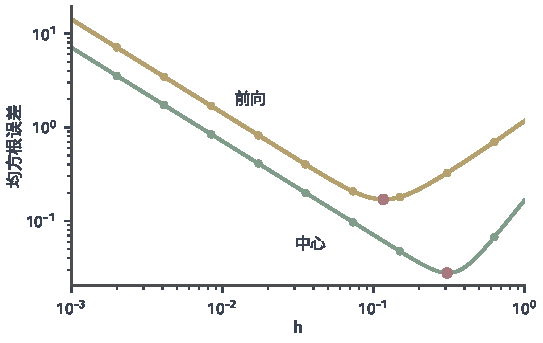
\includegraphics[width=92mm]{figures/05-optimization/05-stochastic-optimization/matplotlib/zo-tradeoff/figure.pdf}
  \caption{差商均方根误差随$h$的变化，$\varphi(s)=s^2/2+s^3/6$，$s_0=1$，独立噪声$\sigma=0.01$。黄线为前向差分，绿线为中心差分，曲线是偏差平方加方差的精确值，圆点是$2\times10^5$次模拟的结果，红点是各自的最小值。$h$小时两线斜率都是$-1$，$h$大时分别是$1$和$2$。}
  \label{fig:zo-tradeoff}
\end{BookInlineFigure}

\paragraph{迭代中的同一取舍}
在迭代算法中，平滑半径受同样的取舍支配，但记账的单位变了。定理~\ref{thm:zo-convex}的上界对$\delta$的依赖是$\alpha V+L\delta^2/2$，而$V$里的噪声项$\propto1/\delta^2$。

图~\ref{fig:zo-delta-u}用一个非二次的凸目标$f(\bm{x})=\sum_{i=1}^2(e^{x_i}-x_i-1)$做实验，解是原点，$f^\star=0$，算法跑固定轮数，噪声$\sigma=0.2$。$\delta$小的一侧，误差按$1/\delta^2$增长，来自噪声；$\delta$大的一侧，平滑目标的解偏离原点，误差快速上升。最好的$\delta$在$0.5$附近，目标差约$0.0026$，$\delta=0.02$和$\delta=4$时都超过$1$。

\begin{BookInlineFigure}
  \centering
  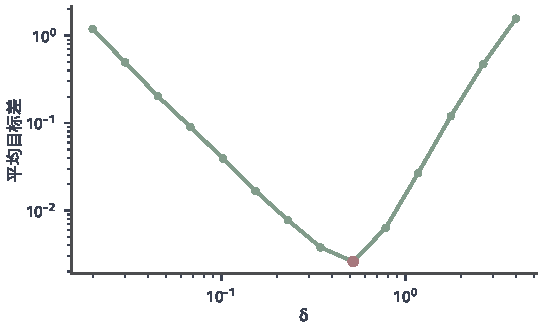
\includegraphics[width=92mm]{figures/05-optimization/05-stochastic-optimization/matplotlib/zo-delta-u/figure.pdf}
  \caption{双点方法在$f(\bm{x})=\sum_{i=1}^2(e^{x_i}-x_i-1)$上的平均目标差随$\delta$的变化，起点$(1,1)$，$\alpha=0.02$，$\sigma=0.2$，$T=3000$，取最后$500$步的平均，$200$次运行。左支由噪声放大主导，右支由平滑偏差主导，红点是扫描到的最小值。}
  \label{fig:zo-delta-u}
\end{BookInlineFigure}

\paragraph{共享样本时规律不同}
上面的$1/\delta^2$规律只适用于独立加性噪声。共享的Lipschitz样本下，差商的方差不随$\delta$增大而爆炸，$\delta$可以尽量取小，U形曲线的左支几乎消失。而指示函数样本的方差$\propto1/\delta$，左支依然存在，只是坡度减半。用哪个$\delta$要先确定噪声模型。

\subsection{维数与方向数}
\label{sec:zo-dimension}

“每轮只读两次”常被误解成成本与维数无关。上面的$\alpha\lesssim1/(nL)$已经说明，维数并没有消失，只是从每轮的读数次数转移到了步长上。

\paragraph{单轮比较}
表~\ref{tab:zo-moments}比较完整坐标差分和随机方向在单轮的成本与误差。这里的“方向波动”是读数精确时二次函数上的$\mathbb{E}\lVert\hat{\bm{g}}-\bm{g}\rVert_2^2$。

\begin{BookInlineTable}
  \centering
  \begin{tabular}{@{}llll@{}}
    \toprule
    方法 & 单轮读数 & 方向波动 & 独立噪声贡献\\
    \midrule
    中心坐标 & $2n$ & $0$ & $n\sigma^2/(2h^2)$\\
    单方向对称 & $2$ & $(n-1)\lVert\bm{g}\rVert_2^2$ & $n^2\sigma^2/(2\delta^2)$\\
    $m$方向对称 & $2m$ & $(n-1)\lVert\bm{g}\rVert_2^2/m$ & $n^2\sigma^2/(2m\delta^2)$\\
    $m$方向共用中心 & $m+1$ & 取决于函数 & $2n^2\sigma^2/(m\delta^2)$\\
    \bottomrule
  \end{tabular}
  \caption{一轮估计的成本与误差。$m=n$时，随机方向的噪声贡献与中心坐标差分相同，都是$n\sigma^2/(2\delta^2)$，读数次数也相同。}
  \label{tab:zo-moments}
\end{BookInlineTable}

\paragraph{相同预算下的结果}
图~\ref{fig:zo-dims}在$n=20$的二次目标上比较三种配置，步长按单轮二阶矩调节：坐标差分用$1/L$，$m$方向平均用$1/(L(1+(n-1)/m))$。横轴都是函数读数次数。读数精确时三条线基本平行，图(a)；读数含噪时停在几乎同一水平，图(b)。

\begin{BookInlineFigure}
  \centering
  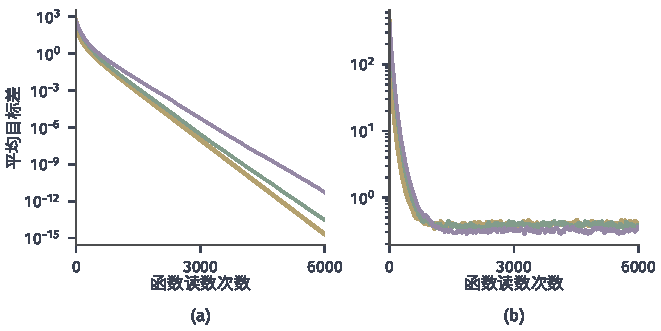
\includegraphics[width=112mm]{figures/05-optimization/05-stochastic-optimization/matplotlib/zo-dims/figure.pdf}
  \caption{$n=20$的二次目标，$\bm{H}$的对角元从$1$均匀到$9$，$h=\delta=0.1$，$30$次运行平均。黄线：中心坐标差分。绿线：$m=1$的随机方向。紫线：$m=5$的随机方向。(a)读数精确。(b)独立噪声$\sigma=0.1$。按读数次数计，三者的差别远小于“两次查询对$40$次查询”的字面差距。}
  \label{fig:zo-dims}
\end{BookInlineFigure}

这个实验的结论有范围。它说明在按读数计费、读数可独立提交的情形下，每轮少读并不等于总成本少。随机方向的优势在别处：可以在读完所有坐标之前就开始移动。梯度集中在少数方向时效果可能更好，但这取决于具体结构，本章没有相应的定理。反过来，如果读数可并行、每轮墙钟时间固定，完整差分反而可能更快。

\paragraph{方向平均与共用中心读数}
独立方向平均把方差除以$m$，这部分依赖独立性。为节省读数，有人让所有方向共用一次中心读数$y_0=f(\bm{x})+\zeta_0$，读数次数从$2m$降到$m+1$。这时
\[
 \hat{\bm{g}}=\frac{n}{\delta m}\sum_{j=1}^m(y_j-y_0)\bm{u}_j,
\]
噪声部分是$\tfrac{n}{\delta m}\sum_j(\zeta_j-\zeta_0)\bm{u}_j$。给定方向，$\zeta_0$对所有方向是同一个数，噪声不再独立，二阶矩是
\[
 \frac{n^2\sigma^2}{\delta^2m^2}\Bigl(m+\Bigl\lVert\sum_{j=1}^m\bm{u}_j\Bigr\rVert_2^2\Bigr).
\]
方向独立随机时$\mathbb{E}\lVert\sum_j\bm{u}_j\rVert_2^2=m$，总贡献是$2n^2\sigma^2/(m\delta^2)$，与每方向单独读中心点的情形相同。方向相关时，比如都偏向同一侧，第二项可以高达$m^2$。所以共用中心读数引入了相关性，必须单独计入。

坐标方向上这一点最清楚。前向坐标差分共用$f(\bm{x})$时，噪声的协方差是
\[
 \frac{\sigma^2}{h^2}\bigl(\bm{I}+\bm{1}\bm{1}^\top\bigr),
\]
它的特征值是$(n+1)\sigma^2/h^2$（对应方向$\bm{1}$）和$n-1$个$\sigma^2/h^2$。公共噪声把误差压到一个方向上，如图~\ref{fig:zo-cov}(a)，而中心差分的误差是各向同性的，如图(b)。

\begin{BookInlineFigure}
  \centering
  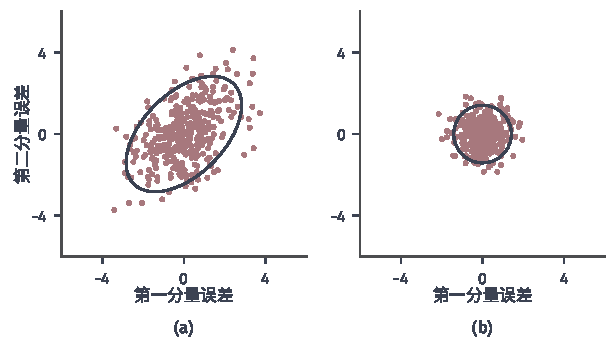
\includegraphics[width=104mm]{figures/05-optimization/05-stochastic-optimization/matplotlib/zo-cov/figure.pdf}
  \caption{$n=2$，$\sigma=h=0.1$时坐标差分的噪声误差。红点是$350$次模拟，黑色椭圆是两倍标准差的等概率线。(a)前向差分共用中心读数，协方差$\begin{bmatrix}2&1\\1&2\end{bmatrix}$，误差沿$(1,1)$方向拉长。(b)中心差分，协方差为$\tfrac12\bm{I}$。}
  \label{fig:zo-cov}
\end{BookInlineFigure}

\subsection{原目标的误差评价}
\label{sec:zo-original-error}

第~\ref{sec:zo-output}节的定理说的都是平滑目标。原来要解决的问题是最小化$f$，本小节补上这一步。

\paragraph{函数平滑误差}
设平滑目标$f_{\mathrm{s}}$与$f$处处至多相差$\gamma_f$，这个常数$\gamma_f$是\term{函数平滑误差}（function smoothing error）。由引理~\ref{lem:zo-smoothing-properties}，光滑函数的球平滑可取$\gamma_f=L\delta^2/2$，$G$-Lipschitz函数可取$\gamma_f=G\delta$。

\begin{theorem}[从平滑目标回到原目标]
\label{thm:zo-transfer}
设$\lvert f_{\mathrm{s}}-f\rvert\leq\gamma_f$，$\bm{x}^\star$是$f$的解，则对任意$\hat{\bm{x}}$，
\begin{equation}
 f(\hat{\bm{x}})-f^\star\leq f_{\mathrm{s}}(\hat{\bm{x}})-f_{\mathrm{s}}(\bm{x}^\star)+2\gamma_f.
 \label{eq:zo-function-transfer}
\end{equation}
若两者的梯度处处至多相差$\gamma_g$（按欧氏范数），则
\begin{equation}
 \lVert\nabla f(\hat{\bm{x}})\rVert_2^2\leq2\lVert\nabla f_{\mathrm{s}}(\hat{\bm{x}})\rVert_2^2+2\gamma_g^2.
 \label{eq:zo-gradient-transfer}
\end{equation}
\end{theorem}

\begin{proof}
由一致误差的假设，
\[
 f(\hat{\bm{x}})\leq f_{\mathrm{s}}(\hat{\bm{x}})+\gamma_f,\qquad f_{\mathrm{s}}(\bm{x}^\star)\leq f^\star+\gamma_f.
\]
两式相加移项得式~\eqref{eq:zo-function-transfer}。

由三角不等式，$\lVert\nabla f\rVert_2$不超过$\lVert\nabla f_{\mathrm{s}}\rVert_2+\gamma_g$，两边平方并用$(a+b)^2\leq2a^2+2b^2$，得式~\eqref{eq:zo-gradient-transfer}。
\end{proof}

式~\eqref{eq:zo-function-transfer}中的$2\gamma_f$在凸函数上可以省一半，因为$f\leq f^{\mathrm{B}}_{\delta}$。把定理~\ref{thm:zo-convex}代回，对光滑凸目标得到
\begin{equation}
 \mathbb{E}f(\bar{\bm{x}})-f^\star\leq\frac{R_0^2}{\alpha T}+\alpha V+L\delta^2.
 \label{eq:zo-convex-original}
\end{equation}
把定理~\ref{thm:zo-nonconvex}代回，取$\gamma_g=L\delta$，对光滑非凸目标得到
\begin{equation}
 \mathbb{E}\bigl\lVert\nabla f(\bm{x}^{(R)})\bigr\rVert_2^2\leq\frac{4\Delta_\delta}{\alpha T}+2L\alpha W+2L^2\delta^2.
 \label{eq:zo-nonconvex-original}
\end{equation}

\paragraph{平滑目标的解不是原目标的解}
这个换算的$\gamma_f$是不能省的。取$f(x)=\max\{x,-2x\}$，$n=1$，$\delta=1$，解是$x^\star=0$。$\lvert x\rvert<1$时，平滑目标的导数是
\[
 \bigl(f^{\mathrm{B}}_{\delta}\bigr)'(x)=\frac{f(x+1)-f(x-1)}{2}=\frac{3x-1}{2},
\]
零点在$x=1/3$，如图~\ref{fig:zo-asym}(a)。平滑目标的精确解带着原目标差$f(1/3)=1/3$。原目标两侧的斜率不对称，平均之后最低点向缓的一侧移动。这笔误差不是算法或噪声造成的，平滑的定义本身就带来了它。

\begin{BookInlineFigure}
  \centering
  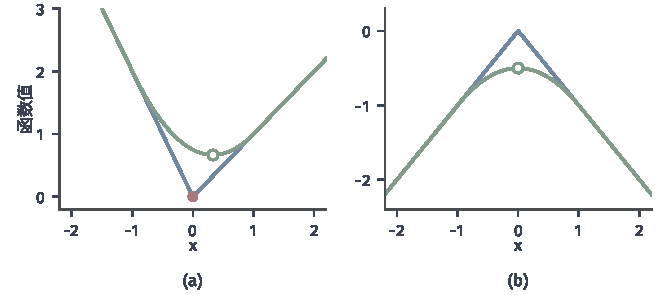
\includegraphics[width=112mm]{figures/05-optimization/05-stochastic-optimization/matplotlib/zo-asym/figure.pdf}
  \caption{平滑目标（绿）与原目标（蓝）的差别，$\delta=1$，一维区间平均。(a)$f(x)=\max\{x,-2x\}$，原解是红点$x=0$，平滑目标的解是空心点$x=1/3$，不在原解上。(b)$f(x)=-\lvert x\rvert$，平滑后在$x=0$处导数为零（空心点），而$x=0$是原函数的极大点。}
  \label{fig:zo-asym}
\end{BookInlineFigure}

\paragraph{原目标不光滑时要换驻点的概念}
式~\eqref{eq:zo-gradient-transfer}需要$\nabla f$存在且$\gamma_g$有限。原目标不可微时，平滑梯度小不能说明原目标梯度小。回到$f=\lvert x\rvert$，由$\bigl(f^{\mathrm{B}}_{\delta}\bigr)'(x)=x/\delta$，在$x=0.01\delta$处平滑导数只有$0.01$，而原函数在此处的导数是$1$。

平滑梯度小给出的是另一种结论。$f$是Lipschitz时，$\nabla f^{\mathrm{B}}_{\delta}(\bm{x})$是$\delta$邻域内各点梯度的平均，所以它小，说明邻域内的梯度有一个小的平均。这是Goldstein意义下的$\delta$驻点，比经典驻点弱。

这也不保证全局最优。图~\ref{fig:zo-asym}(b)的$f=-\lvert x\rvert$，平滑后$x=0$处导数为零，而$x=0$恰恰是原函数的极大点。更一般的多谷目标上，平滑可能磨掉一些浅谷，但没有定理保证平滑目标的驻点在全局最优点附近。

\subsection{函数评估总成本}
\label{sec:zo-total-cost}

\paragraph{成本的组成}
一次优化消耗的函数读数总数是
\begin{equation}
 Q=T\cdot m\cdot q\cdot r+Q_{\mathrm{eval}},
 \label{eq:zo-total-cost}
\end{equation}
其中$T$是迭代轮数，$m$是每轮方向数，$q$是每方向的查询次数，$r$是每个查询点的重复测量次数，$Q_{\mathrm{eval}}$是最终复评的开销。

取$T=200$，$m=2$，$q=2$，$r=3$，末了对$5$个候选各复评$20$次，代入式~\eqref{eq:zo-total-cost}，得到
\[
 Q=200\cdot2\cdot2\cdot3+5\cdot20=2500.
\]
重复测量$r$和扰动尺度$\delta$都能减小差商的噪声，但是方式不同：$r$把方差除以$r$，代价是读数翻$r$倍；增大$\delta$不需要额外读数，但引入偏差。

\paragraph{并行耗时与评估总量}
总量$Q$和实际等待时间是两个量。如果有$12$个并行的仿真槽，上例每轮的$12$次读数可同时提交，迭代部分需要$200$个批次，复评$100$次需要$9$个批次，总共$209$批。单线运行时就是$2500$次。比较算法时要说明用的是哪一个。并行时完整差分的劣势大大减小，甚至可能占优，因为它的每一轮都同时做完。

\paragraph{达到指定精度的成本}
下面把前面的上界解出来，得到达到精度$\varepsilon$所需的读数量级。$\sigma$是独立噪声的标准差。

读数精确且$f$是$L$-光滑凸函数时，由式~\eqref{eq:zo-convex-original}，$V=n^2L^2\delta^2/2$。取$\alpha=1/(4nL)$，上界是
\[
 \frac{4nLR_0^2}{T}+\Bigl(\frac{n}{8}+1\Bigr)L\delta^2.
\]
$\delta$可以任意小，只受浮点精度的限制。取$\delta^2\leq\varepsilon/((2+n/4)L)$，$T=8nLR_0^2/\varepsilon$，每轮两次读数，得到
\[
 Q=\frac{16\,nLR_0^2}{\varepsilon}.
\]
梯度下降需要$O(LR_0^2/\varepsilon)$次梯度，这里多出的正是因子$n$，同完整坐标差分的成本同阶。

独立噪声下，由式~\eqref{eq:zo-convex-original}和$V\approx n^2\sigma^2/(2\delta^2)$，把步长调到最优后上界约为
\[
 2R_0\sqrt{\frac{V}{T}}+L\delta^2=\frac{\sqrt{2}R_0n\sigma}{\delta\sqrt{T}}+L\delta^2.
\]
对$\delta$求最小，得$\delta\propto T^{-1/6}$，误差$\varepsilon\propto T^{-1/3}$，反解$T$得到$Q=O(LR_0^2n^2\sigma^2/\varepsilon^3)$。这里$\delta$必须随预算一起缩小，否则$L\delta^2$这项不消失。这是第~\ref{sec:zo-tradeoff}节U形曲线在迭代算法中的结果。

只有单点反馈且$f$是$G$-Lipschitz凸函数、$\lvert f\rvert\leq B$时，二阶矩是$n^2B^2/\delta^2$，平滑误差是$G\delta$。同样的累加分析给出误差约$R_0nB/(\delta\sqrt{T})+G\delta$，最优化$\delta$后$\varepsilon\propto T^{-1/4}$。

光滑非凸情形按式~\eqref{eq:zo-nonconvex-original}同样处理。精确读数时取足够小的$\delta$，$\alpha=1/(4nL)$，得$Q=O(nL\Delta/\varepsilon^2)$，这里$\Delta$是初始目标与下界之差。独立噪声时平衡$\delta$，得$\varepsilon^2\propto T^{-1/3}$，反解得表中的量级。

表~\ref{tab:zo-costs}汇总这些结果。

\begin{BookInlineTable}
  \centering
  \begin{tabular}{@{}lll@{}}
    \toprule
    反馈与正则性 & 估计器 & 读数量级\\
    \midrule
    精确，$L$-光滑凸 & 双点球面 & $nLR_0^2/\varepsilon$\\
    精确，$L$-光滑非凸 & 双点球面 & $nL\Delta/\varepsilon^2$\\
    独立噪声，$L$-光滑凸 & 双点球面 & $LR_0^2n^2\sigma^2/\varepsilon^3$\\
    独立噪声，$L$-光滑非凸 & 双点球面 & $L^3\Delta n^2\sigma^2/\varepsilon^6$\\
    单点，$G$-Lipschitz凸，$\lvert f\rvert\leq B$ & 单点球面 & $n^2R_0^2B^2G^2/\varepsilon^4$\\
    共享Lipschitz样本，凸 & 双点球面 & $n^2G^2R_0^2/\varepsilon^2$\\
    \bottomrule
  \end{tabular}
  \caption{本章简单估计器达到精度$\varepsilon$的读数量级，略去常数。凸问题的精度指目标差，非凸问题指$\lVert\nabla f\rVert_2\leq\varepsilon$；末行由$\lVert\hat{\bm{g}}\rVert_2\leq nG$的粗略界得到。这些都是上界，不是问题本身的下界。}
  \label{tab:zo-costs}
\end{BookInlineTable}

表的最后一行可以改进。利用球面上Lipschitz函数的集中不等式，双点估计的二阶矩能够改进到$O(nG^2)$，读数量级相应地变成$nG^2R_0^2/\varepsilon^2$。这一步的证明需要用到球面集中不等式，篇幅较长，读者可查阅Duchi等人及Shamir关于双点反馈的工作。它的含义是：共享样本下，配对的收益是把维数从平方降到一次方。

比较时要留意三件事。一是接口：表中的噪声列不能跨行混用，独立噪声的速率不适用于共享样本，反之亦然。二是度量：目标差和梯度范数的$\varepsilon$不是一回事。三是假设：更好的指数往往需要更强的光滑性和更复杂的估计器，不是换一个步长就能得到。
